
%
\documentclass[%
 reprint,
 amsmath,amssymb,
 aps,
]{revtex4-1}

\usepackage{graphicx}% Include figure files
\usepackage{dcolumn}% Align table columns on decimal point
\usepackage{bm}% bold math


\begin{document}



\title{Sistema de Gestion para el concurso de Proyectos de la EPIS}
\author{Jose Pastor Mendoza}
\author{Arlyn Cotrado Coaquira}
\author{Andrés De La Barra Vasquez}
\affiliation{%
 Universidad Privada de Tacna \textbackslash Facultad de Ingenieria \textbackslash Escuela Profesional de Ingenieria de Sistemas
}%

\begin{abstract}
\begin{center}
\textbf{Resumen}
\end{center}
Debido a que usan diferentes herramientas durante la gestión del concurso de proyectos de Escuela Profesional de Ingeniería de Sistemas de la Universidad Privada de Tacna, se desarollará un sistema web denominado "Sistema de Gestión de Proyectos para la EPIS" donde se pueda realizar dicha gestión y unificar los procesos.


\begin{center}
\textbf{Abstract}
\end{center}
Because they use different tools during the management of the project contest of the Professional School of Systems Engineering of the Private University of Tacna, a web system called "Project Management System for EPIS" will be developed where said management and unify processes.

\end{abstract}



\maketitle

%\tableofcontents

\section {Introducción}

El presente proyecto va referido al rubro de educación universitaria; se observó que en la Escuela Profesional de Ingeniería de Sistemas realizan algunos procesos de manera no automatizada para la gestión del concurso de proyectos, haciendo uso tambien de diferentes herramientas.
Este proyecto se justifica por el beneficio que implica para los estudiantes, administradores y para los jurados.

\section{Autores}
\begin{itemize}
\item José Edilberto, Pastor Mendoza.
\item Arlyn Cotrado Coaquira
\item Andrés De La Barra Vasquez
\end{itemize}

\section{Planteamiento del problema}
\subsection{Problema}
No tener un estructura definida en los concursos liberados en la universidad privada de tacna, la necesidad de poder gestionarlo con más herramientas y más procesos se ve necesaria para poder establecer informes y un control avanzado de ello. 
Se converso con la ingeniería Liliana respecto a la problemática respecto a la gestión del concurso de proyectos de la EPIS y nos indico que actualmente no se cuenta con un sistema especifico para esta actividad, por lo que deben recurrir al uso de Excel, Gmail, un software online solo para realizar sorteos, asi como también implementar algunas funciones extras para realizar la calificación de proyectos por parte de los jurados y sobretodo, unificar estos procesos.

\subsection{Justificacion}
Hoy en día las empresas necesitan tecnologia para que sus empleados sean eficientes en su trabajo, de esta manera pueden beneficiarce para obtener una mejor calidad de servicio, mejorar sus procesos y por consiguiente clientes satisfechos.

\subsection{Alcance}
El proyecto se realizara para la gestion de concursos de proyectos en la escuela de la epis, que tendran los modulos de revision, sorteo, categorias, cursos, docentes, creacion de eventos y el seguimiento de votos para la gestion de el concurso de proyectos. 

%-----------------------------------------------------------------
\section {Objetivos}
\subsection {General}
Integrar todas las actividades involucradas en el proceso del concurso de proyectos de la EPIS.
\subsection {Especificos}
\begin{itemize}
\item Facilitar a todos los usuarios el proceso que les corresponda realizar segun su rol. \\
\item Investigar el uso de tecnologias web para la realizacion del proyecto.  \\
\item Crear un producto completo para mejorar tiempos y organizar procesos .\\
\end{itemize}

\section {Desarrollo de la propuesta}
La presente propuesta plantea:
\begin{itemize}
    \item Realizar una aplicación web que contenga 3 vistas: 1 para los estudiantes, otra para el administrador del concurso de proyectos (Ingeniera Liliana) y otra para los jurados.
     \item Para la vista del estudiante, tendrá que crearse una cuenta , luego tendrá una vista sobre información respecto al concurso de proyectos(documentos que necesite) y también, un modulo para subir toda la documentación y registrar su proyecto que será enviado a evaluar por el administrador.
     \item Para la vista del administrador, tendrá un modulo para ver las solicitudes de los proyectos que desean registrarse para participar. Tendra otro modulo para organizar que categorías y que cursos van a participar. Otro modulo será para agregar a los jurados para cada categoría. Otro modulo para hacer un seguimiento de votos. 
    \item Para la vista del jurado, solo tendrán el modulo para votar según la categoría a la que esten asignados.
    \item Tambien se plantea agregar un chatbot al Facebook de Tutoria Epis, la cual se encargara de dar información histórica sobre el concurso de proyectos (referido a información del pasado sobre los ganadores de anteriores ediciones, nombres de proyectos que hayan participado).
\end{itemize}
\newpage
Tecnologias que usaremos :
\begin{itemize}
\item Laravel :
Laravel es un framework de código abierto para desarrollar aplicaciones y servicios web con PHP 5 y PHP 7. Su filosofía es desarrollar código PHP de forma elegante y simple, evitando el "código espagueti". Fue creado en 2011 y tiene una gran influencia de frameworks como Ruby on Rails, Sinatra y ASP.NET MVC
\item Reactjs :
React es una biblioteca Javascript de código abierto diseñada para crear interfaces de usuario con el objetivo de facilitar el desarrollo de aplicaciones en una sola página. Es mantenido por Facebook y la comunidad de software libre. Han participado en el proyecto mas de mil desarrolladores diferentes.
\item MySQL o PostgreSQL:
PostgreSQL, también llamado Postgres, es un sistema de gestión de bases de datos relacional orientado a objetos y de código abierto, publicado bajo la licencia PostgreSQL.
\end{itemize}
\begin{center}
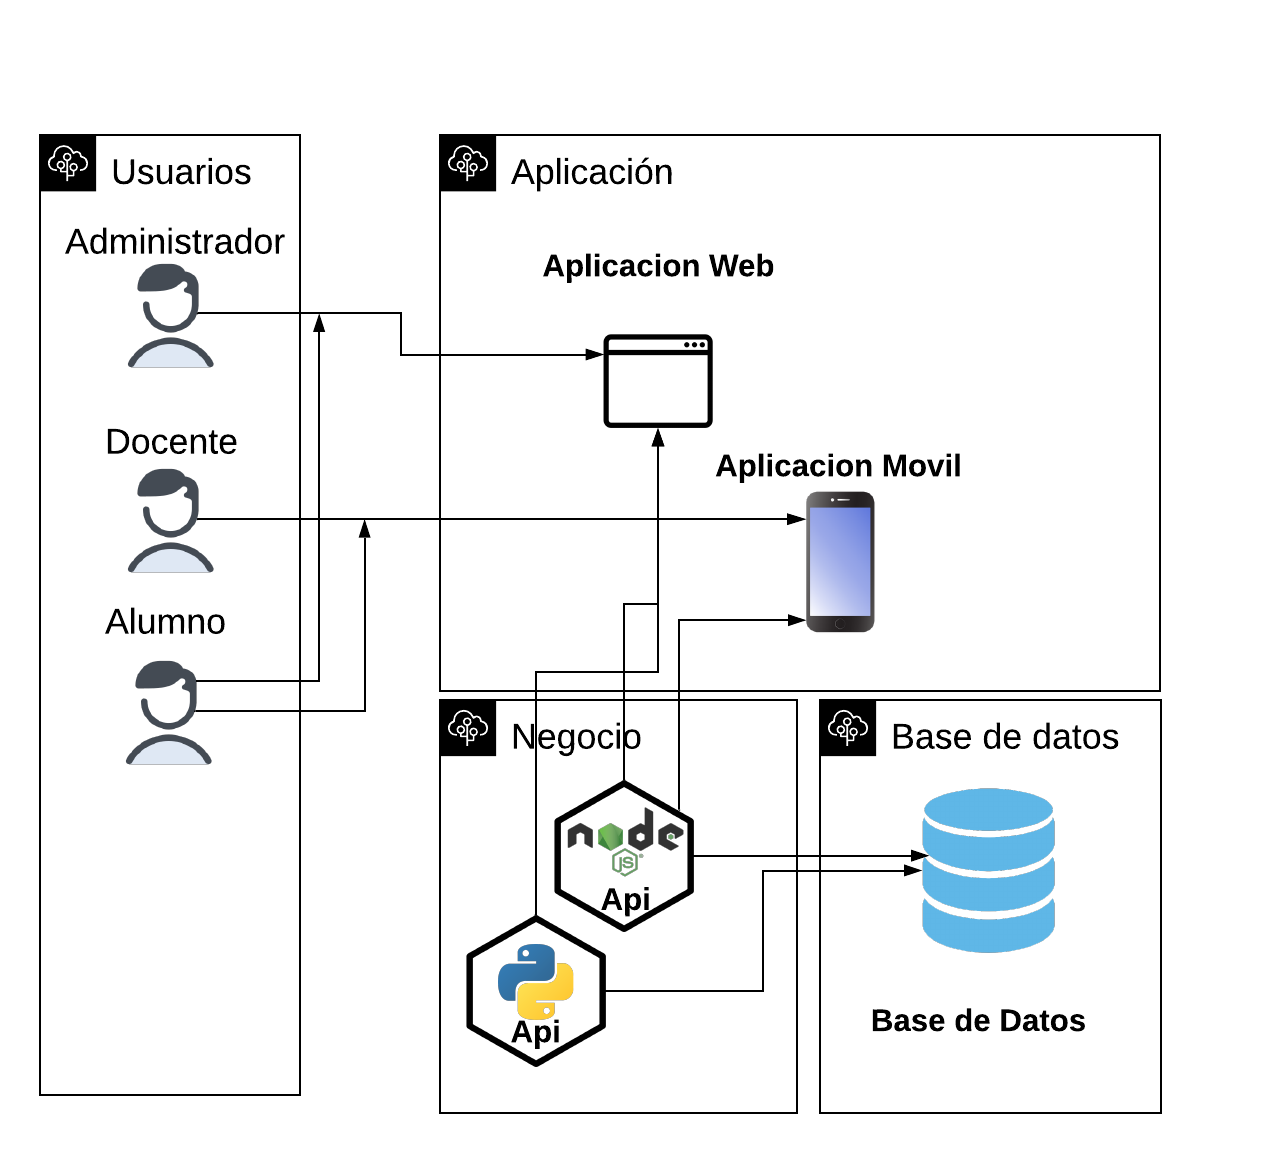
\includegraphics[width=10cm]{./Imagenes/arquitectura2}
\end{center}

%-----------------------------------------------------------------
\section{Conclusiones}

\begin{itemize}
\item La presente propuesta resuelve e integra las actividades totales que conlleva la realización del concurso de proyectos de la EPIS, tales como la inscripción de los participantes, organización de los equipos y también calificación de los jurados. 

\item La implentacion de una funcionalidad extra, que es la posibilidad de los estudiantes espectadores  para votar por el proyecto que más simpatizan,  solicitada por la organizadora del concurso como una posibilidad a implementar a futuro. 

\item Las tecnologías web a aprender y desarrollar durante el proceso del proyecto involucran la actualización e investigación por parte del grupo de trabajo, lo cual cumple uno de los objetivos principales como estudiantes de la carrera de Ingenieria de Sistemas, el cual es ser autodidactas y buscar la constante capacitacion, al tener tecnologias renovadas cada dia.
 

\end{itemize}

% Bibliografia.
%-----------------------------------------------------------------

%\bibliographystyle{plain}
%\bibliography{Bibliografia}

\end{document}

